% !TeX root = ../../../book.tex
\section{学而时习之}\label{sec:section1.5}

我们以一些练习结束本章,这些练习既包含讨论过的概念,又能让你实践所学知识,同时可以让你保持思维敏捷。请尽可能尝试解答,并与朋友探讨解题思路。不过,归根结底,把这些练习当作一种保持大脑灵活的方式就好!\\

\begin{exercise}
    一只苍蝇停在一辆以 $60$ 公里/小时的速度行驶的火车前端。同轨道前方 $300$ 公里处,另一列火车正以 $60$ 公里/小时的速度迎面驶来。当两车相距 $300$ 公里时,苍蝇以 $90$ 公里/小时的速度起飞,在火车间的轨道上来回飞行,到达火车时瞬间转向。当两车相撞挤压苍蝇时,苍蝇共飞行了多少距离?你是如何求解的?尝试推广到一列火车时速 $a$ 公里,另一列火车时速 $b$ 公里,苍蝇时速 $c$ 公里。
\end{exercise}

\begin{exercise}
    政府铸币厂受委托铸造一批金币。铸币厂有 $20$ 台机器,每台机器生产重 $5$ 克的金币。某日工头发现部分金币偏轻,经检查发现有一台机器铸造出的金币为 $4$ 克,其余 $19$ 台机器正常。他决定化不利为有利,借此选拔最聪明的员工进行提拔。工头告知工人:仅有一台机器生产的金币为 $4$ 克,且仅允许用秤称量一次。作为员工,你可选取任意选定机器生产的任意数量的金币,但需合并称重并读取总克数。如何准确找出故障机器?
\end{exercise}

\begin{exercise}
    在国际象棋中,皇后可以沿垂直、水平或对角线方向移动任意格数。在标准 $8 \times 8$ 棋盘上放置 $8$ 个皇后,要求任意皇后均无法攻击其他皇后(即\emph{不存在}皇后可在一步内吃掉另一皇后)。请给出一种解法或证明其不可能性。若存在解法,试讨论共有多少种不同放置方式;若不可能,请确定棋盘上最多可放置多少个满足条件的皇后。
\end{exercise}

\begin{exercise}
    在标准 $8 \times 8$ 棋盘上去除对角位置的两个方格(例如左上角和右下角)。能否用 $2 \times 1$ 多米诺骨牌不重叠地覆盖所有剩余方格(即实现棋盘\emph{密铺})?请说明理由。推广至 $n \times n$ 棋盘,该结论是否依赖 $n$ 的取值?请解释原因。
\end{exercise}

\begin{exercise}
    考虑标准 $8 \times 8$ 棋盘,移除两个相邻的对角方格(如图所示)。能否用 T 形四联骨牌密铺该棋盘?若可行,请描述方法;若不行,请解释原因。

    \begin{center}
        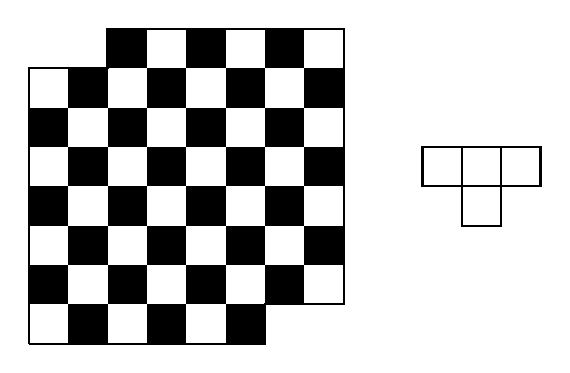
\begin{tikzpicture}[thick, scale=0.5, x=1cm]
            \foreach \x in {0,...,5}
                {
                    \pgfmathparse{mod(\x,2) ? "black" : "white"}
                    \edef\colour{\pgfmathresult}
                    \path[fill=\colour] (\x, 0) rectangle ++ (1,1);
                }
            \foreach \x in {0,...,7} 
                \foreach \y in {1,...,6}
                    {
                        \pgfmathparse{mod(\x+\y,2) ? "black" : "white"}
                        \edef\colour{\pgfmathresult}
                        \path[fill=\colour] (\x,\y) rectangle ++ (1,1);
                    }
            \foreach \x in {2,...,7}
                {
                    \pgfmathparse{mod(\x+1,2) ? "black" : "white"}
                    \edef\colour{\pgfmathresult}
                    \path[fill=\colour] (\x, 7) rectangle ++ (1,1);
                }
            \draw (0,0)--(6,0)--(6,1)--(8,1)--(8,8)--(2,8)--(2,7)--(0,7)--(0,0);
            \draw (10,4) rectangle ++ (1,1);
            \draw (11,4) rectangle ++ (1,1);
            \draw (12,4) rectangle ++ (1,1);
            \draw (11,3) rectangle ++ (1,1);
        \end{tikzpicture}
    \end{center}
    推广至 $n \times n$ 棋盘,该结论是否依赖 $n$ 的取值?请说明理由。
\end{exercise}

\begin{exercise}
    给定实数 $x$,定义 $\lfloor x \rfloor$ 为小于或等于 $x$ 的最大整数,$\lceil x \rceil$ 为大于或等于 $x$ 的最小整数。例如,$\lfloor 6.02 \rfloor = 6, \lfloor 6.99999 \rfloor = 6, \lfloor 6 \rfloor = 6, \lfloor -6.5 \rfloor = -7$。尽可能为以下表达式的值找到更具体和简洁的表示形式。(你可能需要根据 $x$ 的值给出不同表达式。)

    \begin{enumerate}
        \item $\lfloor x \rfloor + \lfloor 1-x \rfloor$ 
        \item $\lceil x \rceil + \lceil 1-x \rceil$
        \item $\lfloor x \rfloor + \lceil x \rceil$
        \item $\frac{\lfloor x \rfloor}{x}$
        \item $\lfloor x^2 \rfloor - \lfloor x \rfloor ^2$
        \item $\lceil x^2 \rceil - \lceil x \rceil^2$
    \end{enumerate}
\end{exercise}

\begin{exercise}
    求三个自然数 $a,b,c$,使得没有子集之和能被 $3$ 整除。即求 $a,b,c$ 满足以下和均不被 $3$ 整除:$a,b,c,a + b,a + c,b + c,a + b + c$。这可能吗?为什么?\\
    \\
    尝试用 $4$ 个数做同样的事:求自然数 $a,b,c,d$,使得没有子集之和能被 $4$ 整除。这可能吗?为什么?\\
    \\
    尝试推广:你能说明如何找到 $n$ 个自然数,使得所有子集之和都不能被 $n$ 整除吗?
\end{exercise}

\begin{exercise}
    回顾通过点和彩色连线解决朋友倾向问题的方法。这里我们考虑类似情形:给定若干点,需绘制所有可能线段,使得任意两点恰由一条线段连接,但忽略颜色(所有线段可视为黑色)。你能用 $3$ 个点画出该图形且所有线段不交叉吗?$4$ 个点呢?$5$ 个点呢?$6$ 个点呢?为什么可以或为什么不可以?尝试解释为什么某些图形不可能实现。若无法达成 $0$ 次交叉,可能达到的最小交叉次数是多少?
\end{exercise}

\begin{exercise}
    画一个圆,沿圆周放置 $3$ 个点。现需对点之间的圆弧着色(每段一种颜色),要求相邻圆弧的颜色不同。至少需要多少种颜色?若放置 $4$ 个点呢?$5$ 个点呢?尝试推广到 $n$ 个点的情况。你能说明所需颜色的最小数量吗?
\end{exercise}

\begin{exercise}
    假设你有一个装满袜子的抽屉,其中有 $2$ 双蓝色袜子、$3$ 双红色袜子和 $4$ 双绿色袜子(左右袜不可区分)。某天清晨你匆忙随机抓取袜子,每次一只,直至手中凑成一双为止。为\emph{保证}获得一双袜子,至少需要从抽屉中取出多少只?\\
    \\
    若每种颜色的袜子数量加倍,答案如何变化?若共有红、绿、蓝、黄、棕五种颜色,每种颜色 $3$ 双呢?推广到 $m$ 种颜色,每种颜色 $n$ 双的情况呢?
\end{exercise}

\begin{exercise}
    深夜,四人行至一座老旧摇晃的桥前。此桥最多同时承载两人,且需手电筒照明。四人过桥所需时间分别为 $5$ 分钟、$10$ 分钟、$15$ 分钟和 $20$ 分钟。两人同行时,按较慢者速度通过。四人全部过桥的最短时间是多少?能否找到绝对最优方案?
\end{exercise}

\begin{exercise}
    考虑美元硬币的常见面额:$1$ 美分、$5$ 美分、$10$ 美分和 $25$ 美分。为\emph{保证}能精确支付 $0$ 到 $100$ 美分间的任意金额,口袋中至少需携带哪些硬币?是否存在多组可行方案?满足此要求的最小总币值是多少?是否存在总币值相同的最小方案组?
\end{exercise}

\clearpage

\begin{exercise}
    设 $a,b,c$ 为实数且 $a \ne 0$。以下关于方程 $ax^2 + bx + c = 0$ 解的``伪证明''存在何种错误?\\
    \\
    \textbf{``伪证明'':}设 $x$ 与 $y$ 为方程的解。由 $ax^2+bx+c = 0$ 减 $ay^2+by+c = 0$ 得 $a(x^2-y^2)+b(x-y) = 0$。因式分解得 $a(x+y)(x-y)+b(x-y) = 0$,故 $a(x+y)+b = 0$,即 $x + y = -\frac{b}{a}$。由于 $x$ 和 $y$ 是\emph{任意}解,可令 $x = y$ 代入得 $2x = -\frac{b}{a}$,故 $x = -\frac{b}{2a}$ 为解。``$\square$''
\end{exercise}

\begin{exercise}
    请解释为什么 $(-1)(-1) = 1$。假设你正在为一位对此事实持怀疑态度的同学撰写说服性证明,该同学与你智力水平相当,禁止仅回答``定义如此''。尝试构建\emph{几何}或\emph{物理}解释,或提出令人信服的论证。
\end{exercise}

\begin{exercise}
    求下列方程的所有实数解:

    \begin{enumerate}
        \item $\vert x-2 \vert = \vert x-3\vert$
        \item $\vert 2x-1 \vert = \vert 2x-3\vert$
        \item $\vert 2x-2 \vert = \vert 2x-3\vert$
        \item $\vert x+1 \vert = \vert x-5\vert$
        \item $\vert x-1 \vert + \vert x-2 \vert = \vert x-3\vert$
    \end{enumerate}
\end{exercise}

\begin{exercise}
    \textbf{逻辑俱乐部第一规则...:}要想加入逻辑俱乐部,必须选择\emph{始终}说真话或\emph{始终}说谎话。逻辑俱乐部的成员知道谁说谎,谁诚实。我不是逻辑俱乐部的成员,但我在街上遇到三名成员发表了以下言论:
    \begin{itemize}
        \item 杰克:``我们三个都是骗子。''
        \item 泰勒:``我们三人中只有两人是骗子。'' 
        \item 查克:``杰克和泰勒是骗子。''
    \end{itemize}
    那么,我应该相信谁呢?
\end{exercise}

\begin{exercise}
    求解满足方程 $\sqrt{x - 1} = x - 3$ 的所有实数解。展示解题过程,并说明为什么只有\emph{唯一}解。
\end{exercise}

\begin{exercise}
    你有两根保险丝,每根都能燃烧整整一小时。但保险丝不一定相同,且燃烧速率不均匀。你只有一个打火机和这两根保险丝。能否精确测量 $45$ 分钟?如果能,请说明方法;如果不能,请解释原因。
\end{exercise}

\begin{exercise}
    本题改编自 1926 年《星期六晚邮报》上的经典谜题!\\
    \\
    三个朋友凑钱买了一大袋 \text{M\&M} 糖果。他们把糖果带回公寓,决定第二天在聚会上分享。夜里,第一个人醒来想吃零食。他决定提前吃掉自己那份。他打开袋子,将糖果分成三等份,发现多出一粒。他认为多吃一粒无妨,便吃掉了自己的那份和多余的一粒,然后将剩余糖果放回袋子。过了一会儿,第二个人醒来做了同样的事:把袋中剩余糖果分成三份,吃掉了自己的那份和多余的一粒。又过了一会儿,第三个人也如法炮制,吃掉了自己的那份和多余的一粒。第二天聚会时,他们将最后剩余的糖果均分成三份享用(当然无人承认前夜所为)。\\
    \\
    问:最初袋中最少可能有多少颗 \text{M\&M} 糖果?
\end{exercise}

\begin{exercise}
    给定一个实数列表,其\emph{算术}平均数定义为总和除以项数,其\emph{几何}平均数定义为乘积的项数次方根。也就是说,假设设 $x_1, x_2, \dots , x_n$ 为实数,则算术平均数为
    \[\frac{x_1+x_2+ \dots + x_n}{n}\]
    几何平均数为
    \[\sqrt[n]{x_1 \cdot x_2 \cdot \dots \cdot x_n}\]
    (注意:一个数的 $n$ 次方根等于该数的 $\frac{1}{n}$ 次方。)
    \\
    能否找到两个数,使其算术平均数与几何平均数\emph{相等}?能否找到两个数,使其算术平均数严格大于几何平均数?反之呢?
    \\
    取三个数、四个数等重复上述操作。你能总结出一般规律吗?
\end{exercise}

\begin{exercise}
    考虑不定方程 $6x + 15y = 93$。我们希望求其\emph{整数}解;也就是说,我们想找到满足方程的 $x$ 和 $y$ 的\emph{整数}(自然数、零和负自然数)解。

    \begin{enumerate}
        \item 找出一组 $x$ 和 $y$ 均为正整数的解,并简述求解方法。
        \item 找出一组 $x$ 或 $y$ 中一个为正、另一个为负的解,并说明求解过程。
        \item 你认为该方程有多少组解?尝试刻画所有解的表达式或描述求解思路。
    \end{enumerate}
\end{exercise}

\begin{exercise}
    \textbf{幻方}是一个 $n \times n$ 数组,包含 $1$ 至 $n^2$ 的所有整数,且满足每行、每列及两条主对角线的数字之和均相等(该和称为\textbf{幻数和})。例如,下面是一个幻数和为 $15$ 的 $3 \times 3$ 幻方:
    \begin{center}
        \begin{squarecells}{3}
            8 & 1 & 6 \nl
            3 & 5 & 7 \nl
            4 & 9 & 2 \nl
        \end{squarecells}
    \end{center}
    能否推导出 $n \times n$ 幻方的幻数和公式?
    \\
    (提示:我们在本章中发现过一个有用的结论。)
\end{exercise}

\begin{exercise}
    小于或等于 $1000$ 的整数中,有多少整数至少有一位为 $1$?例如 $1$、$12$ 和 $511$。
\end{exercise}

\begin{exercise}
    现有若干堆考拉熊(每堆视为一个集合)。操作规则为:从每堆取出一项,将所有取出项合并为新堆。例如:
    现有若干堆考拉熊。为了打散它们,我们从每堆中取出一只考拉熊,然后将所有这些考拉熊放入新的一堆中。例如,如果我们从大小为 $1$、$4$ 和 $4$ 的考拉熊堆开始,经过一次操作后将得到大小为 $3$、$3$ 和 $3$ 的考拉熊堆;如果我们从大小为 $3$ 和 $4$ 的考拉熊堆开始,经过一次操作后将得到大小为 $2$、$2$ 和 $3$ 的考拉熊堆。\\
    \\
    问:是否存在初始堆配置,使得操作一次后堆的大小(与顺序无关)\emph{保持不变}?\\
    请确定所有满足此性质的初始堆集合,并证明其唯一性。\\
    \\
    \emph{提示 1}:例如初始只有一个大小为 $1$ 的堆,操作后仍为大小为 $1$ 的堆,满足条件。\\
    \emph{提示 2}:需严格证明解的\emph{唯一型},确保无遗漏。
\end{exercise}